\documentclass{beamer}
\usepackage{amsthm}
\usepackage{amssymb}
\usepackage{amsmath}
\usepackage{amsfonts}
\usepackage{graphicx}
\usepackage{tikz}
\usetheme{Rochester}
\usecolortheme{seahorse}
\usefonttheme{structuresmallcapsserif}
\setbeamertemplate{caption}[numbered]
\setbeamertemplate{footline}[frame number]
\usepackage{subfigure}
\newcommand{\myitem}{\item[$-$]}

\title{Efficient segmentation algorithms for shark fin identification}
\subtitle{Honours project proposal by Lize Cilli\'{e}}
\author{Project advisors: Dr. S.J. van der Walt and Prof. B.M.
Herbst}
\date{1 August 2013}
\institute{Department of Applied Mathematics, Stellenbosch University}

\begin{document}
\maketitle


\begin{frame}
\frametitle{Motivation and problem statement}
\begin{itemize}

\item Motivation behind the project.
\begin{itemize}
\myitem Sharks have an unique dorsal fin structure.
\myitem The value of analysing shark fins.
\myitem PhD student in Marine Biology at Stellenbosch University, Ms. Sara
Andreotti.
\myitem Databases of shark fin images that needed to be categorized for studying
behavioural and ecological patterns of sharks.
\myitem Advantage for marine scientists.
\end{itemize}
\item Methodology.
\begin{itemize}
 \myitem We will investigate different methods for classifying the foreground and
background.
 \myitem Segmenting the foreground successfully for matching. 
\end{itemize}

\item Examples of shark fins.
\end{itemize}
\end{frame}


\begin{frame}
\frametitle{Examples of shark fin images showing the unique dorsal part}
\begin{figure}
\centering
\mbox{\subfigure[Shark fin 1]{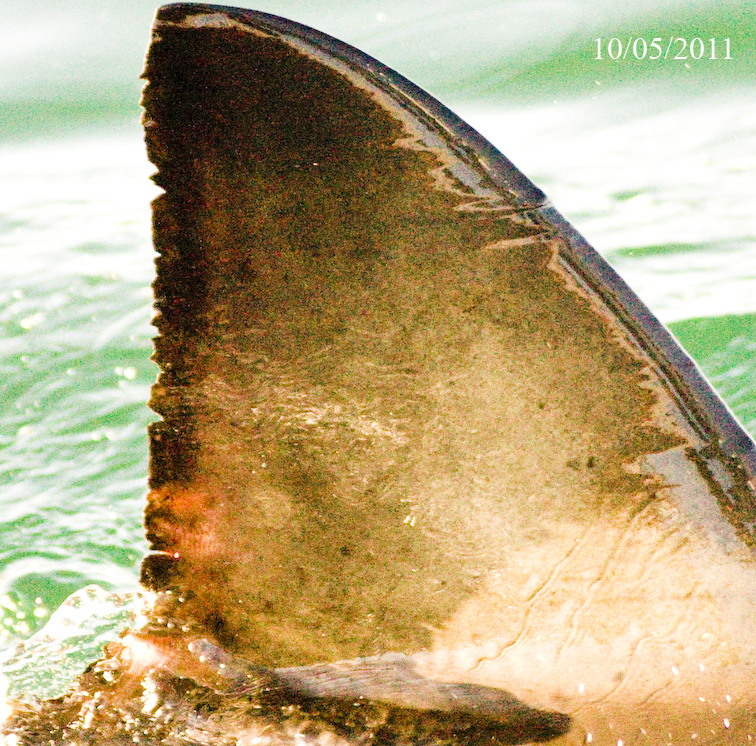
\includegraphics[width=1in]{haai1.jpg}} \quad
\subfigure[Shark fin 2]{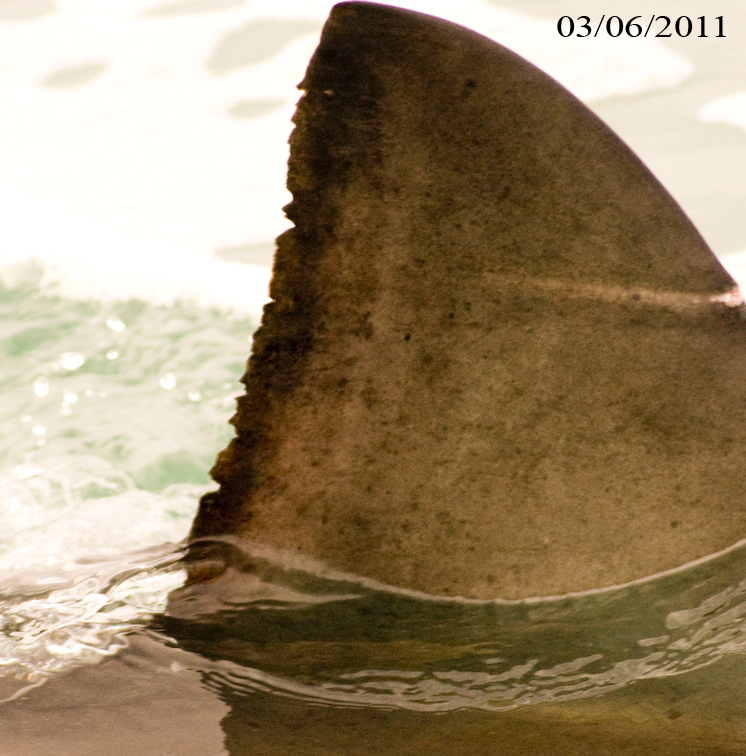
\includegraphics[width=1in]{haai2.jpg}}}
\end{figure}
\begin{figure}
\centering
\mbox{\subfigure[Shark fin 3]{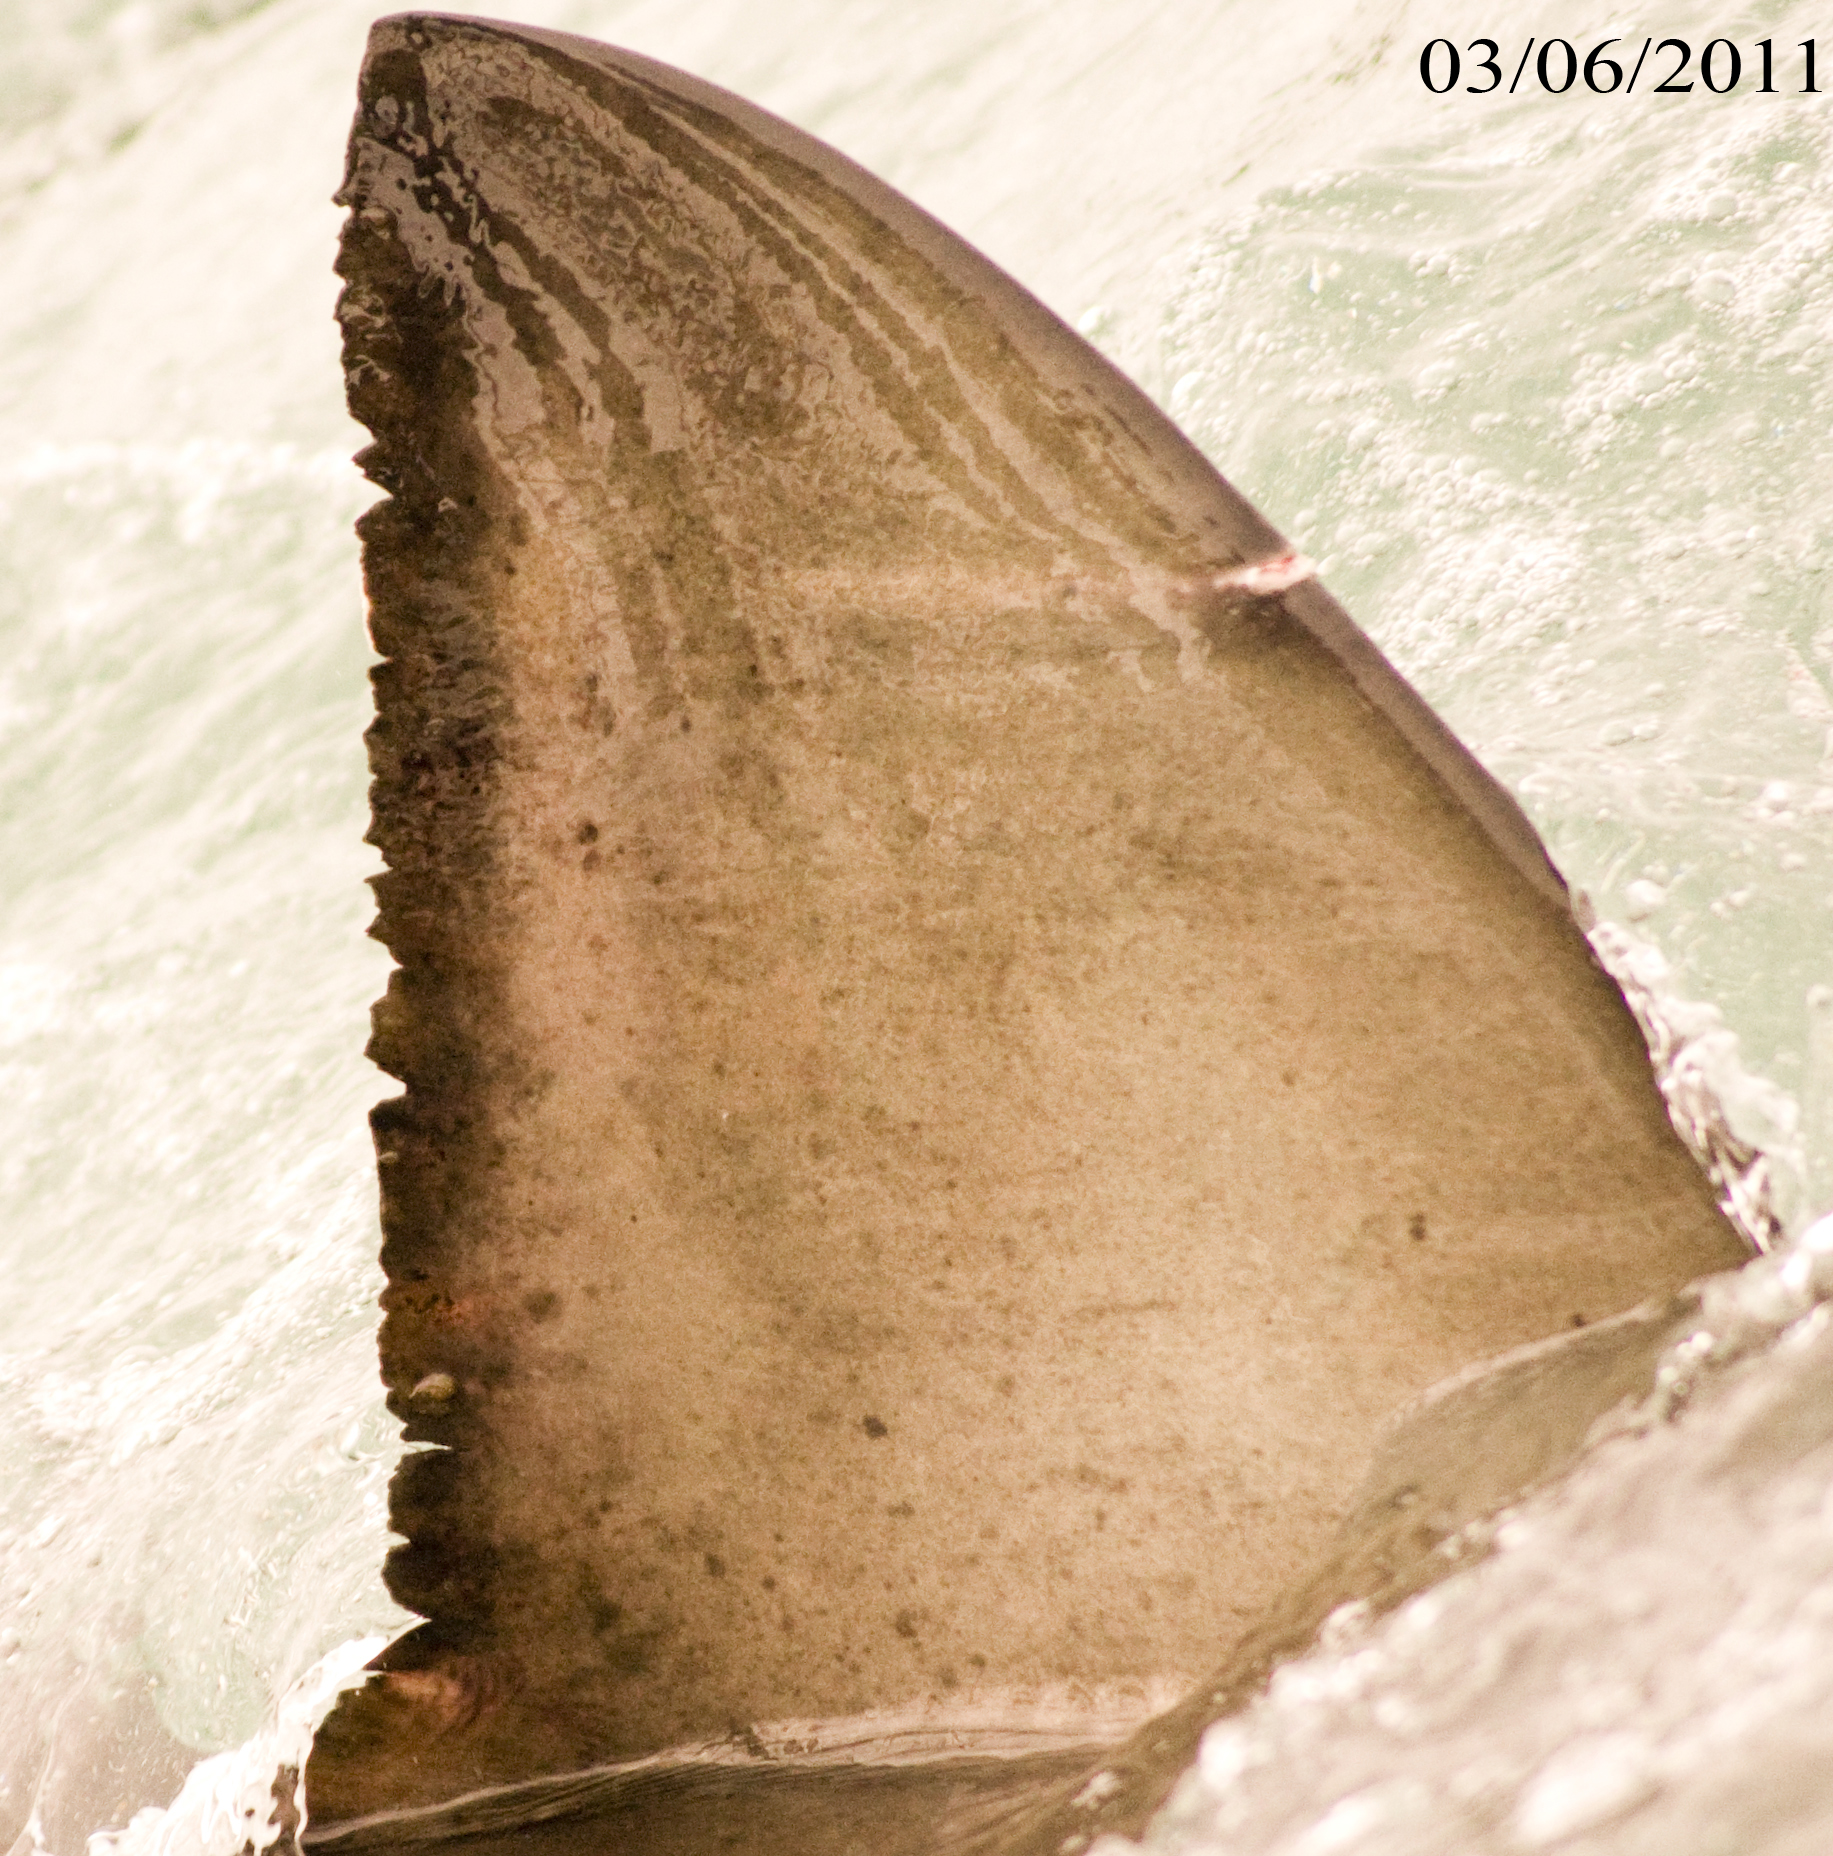
\includegraphics[width=1in]{haai3.jpg}} \quad
\subfigure[Shark fin 4]{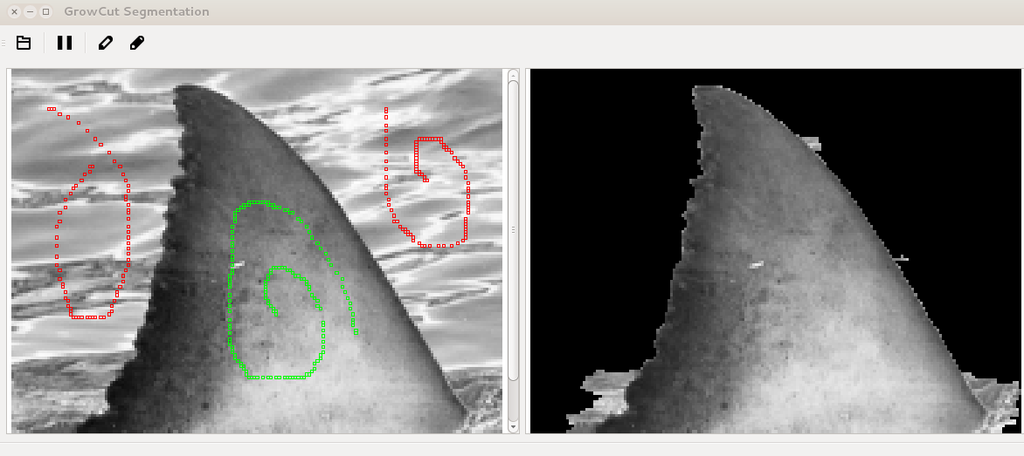
\includegraphics[width=1in]{haaim.png}}}
\end{figure}
\end{frame}


\begin{frame}
\frametitle{Background -- Image segmentation}
\begin{itemize}
\item Basic principle of segmentation algorithms.
\begin{itemize}
\myitem Partitioning a digital image into multiple segments to locate an object or
boundaries in the image.
\end{itemize}
\item Applications.
\begin{itemize}
\myitem Medical imaging to locate tumours.
\begin{figure}
 \centering
 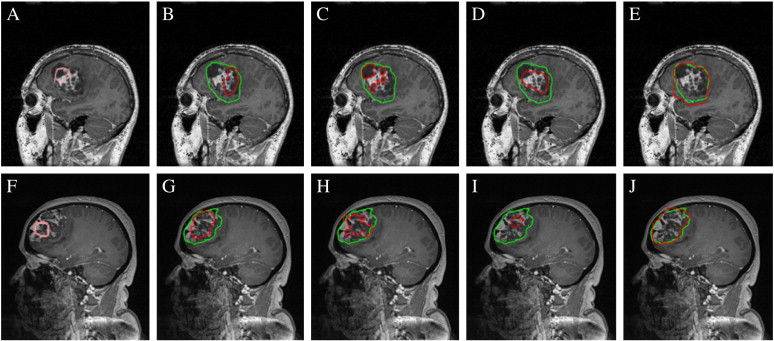
\includegraphics[width=1.7in, height=0.8in]{braintumor.jpg}
 \caption{Braintumours detected by means of image segmentation}
 \end{figure}
\myitem Face and fingerprint recognition.
\myitem Video surveillance.
\end{itemize}
\item Many different techniques.
\end{itemize}
\end{frame}

\begin{frame}
\frametitle{Algorithms from the scikit-image Python library}
\begin{itemize}
\item The Watershed\cite{scikit-image} algorithm.
\item The Random Walker\cite{scikit-image} algorithm.
\end{itemize}
\end{frame}

\begin{frame}
\frametitle{The region growing GrowCut segmentation algorithm}
\begin{itemize}
\item The GrowCut\cite{alg} algorithm is an interactive, multi-label segmentation algorithm for N-dimensional images.
\item How does it work? 
\begin{itemize}
\myitem Cellular Automata\cite{cellularoutomata}.
\myitem Attacking strategies/evolution rule.
\myitem Neighbouring cells 'attack' the cell under consideration.  The state of this cell is then updated
according to the evolution rule.
\end{itemize}
\begin{figure}
\centering
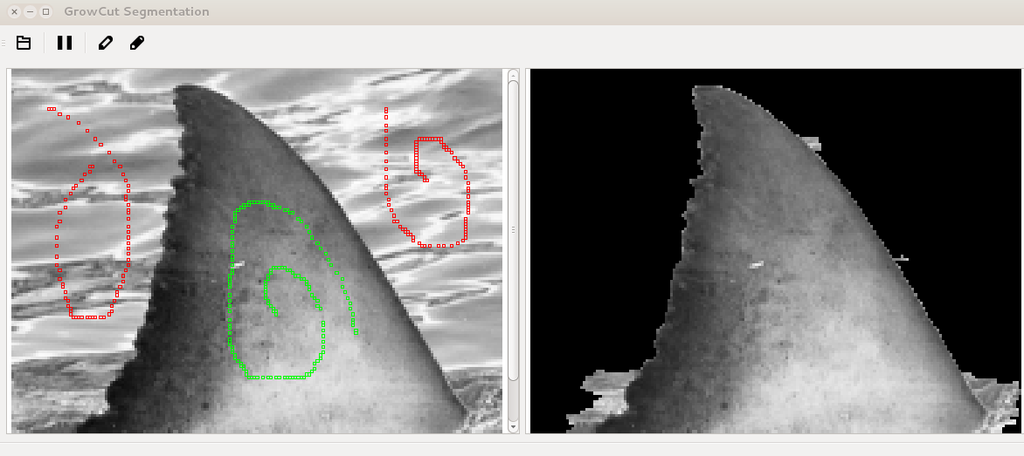
\includegraphics[width=1.7in, height=0.8in]{haaim.png}
\caption{The GrowCut algorithm(GUI by Dr. Nathan Faggian of the Bureau of Meteorology, Australia)}
\end{figure}
\item Success!
\end{itemize}
\end{frame}

\begin{frame}
\frametitle{The region growing GrowCut segmentation algorithm (cont)}
\begin{itemize}
\item Building a pipeline such that the input data is the shark fin image and the output is a specific
classification of that image.
\item Challenges.
\begin{itemize}
\myitem Specification of coordinates.
\end{itemize}
\item Possible solution.
\begin{itemize}
\myitem Orientation.
\end{itemize}
\end{itemize}
\end{frame}


\begin{frame}
\frametitle{DARWIN -- Alternative software}
\begin{itemize}
 \item An article\cite{Darwin} appeared in Die Burger claiming that this
 software could also be used to estimate the size of the Great White shark
 population in the Gansbaai area by means of shark fin identification and
 matching.
 \item The validity of this claim was tested by Ms. Andreotti, which found it to
 be unreliable in 54\% of the cases.
 \item Motivation.
\end{itemize}
\begin{figure}
 \centering
 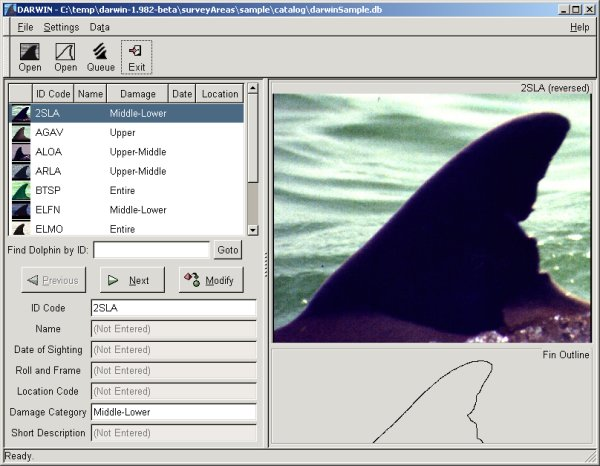
\includegraphics[width=1.5in, height=0.9in]{Darwin.jpg}
 \caption{User interface}
\end{figure}
\end{frame}


\begin{frame}
\frametitle{Conclusions}
\begin{itemize}
\item Future work
\begin{itemize}
 \myitem Attacking strategies.
\end{itemize}
\item Joy and satisfaction of a project of this degree.
\end{itemize}
\end{frame}


\begin{frame}
\frametitle{Bibliography}
\bibliographystyle{plain}
\bibliography{ProjectProposalPresentation}
\end{frame}


\end{document}
